\documentclass[12pt]{article}

\usepackage[a4paper,margin=1in]{geometry}
\usepackage{amsmath,amssymb,amsthm}
\usepackage{tikz}
\usepackage{enumitem}
\usepackage{xcolor}
\usepackage{array}

\setlength{\parindent}{0pt}
\setlength{\parskip}{0.75em}

\newtheorem{definition}{Definition}
\newtheorem{remark}{Remark}
\newtheorem{example}{Example}
\newtheorem{proposition}{Proposition}

\title{Lecture 12: Exponential Interarrival Times, Queues, and Birth-Death Models}
\author{MA4034 -- Time Series and Stochastic Processes}
\date{}

\begin{document}

\maketitle

\section{Construction of a Poisson Process Using Exponential Interarrival Times}

In Lecture 11, we described a Poisson process by counting the number of events in a time interval.

Another useful way to construct a Poisson process is by using the waiting times between consecutive events.

Let
\[
T_1,T_2,T_3,\ldots
\]
be independent and identically distributed exponential random variables with rate \(\lambda\):
\[
T_i\sim \operatorname{Exponential}(\lambda).
\]

Here:
\[
T_1=\text{waiting time until the first event},
\]
\[
T_2=\text{waiting time between the first and second events},
\]
\[
T_3=\text{waiting time between the second and third events},
\]
and so on.

\begin{center}
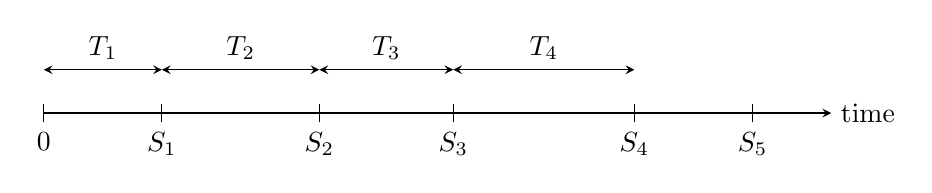
\begin{tikzpicture}[>=stealth, scale=1]
    \draw[->] (0,0) -- (10,0) node[right] {time};
    \foreach \x/\lab in {0/0,1.5/{S_1},3.5/{S_2},5.2/{S_3},7.5/{S_4},9/{S_5}} {
        \draw (\x,0.12) -- (\x,-0.12);
        \node[below] at (\x,-0.12) {\(\lab\)};
    }
    \draw[<->] (0,0.55) -- (1.5,0.55) node[midway,above] {\(T_1\)};
    \draw[<->] (1.5,0.55) -- (3.5,0.55) node[midway,above] {\(T_2\)};
    \draw[<->] (3.5,0.55) -- (5.2,0.55) node[midway,above] {\(T_3\)};
    \draw[<->] (5.2,0.55) -- (7.5,0.55) node[midway,above] {\(T_4\)};
\end{tikzpicture}
\end{center}

Define
\[
S_n=T_1+T_2+\cdots+T_n.
\]

Then \(S_n\) is the time at which the \(n\)th event occurs.

\begin{definition}[Arrival Time]
\[
S_n=T_1+T_2+\cdots+T_n
\]
is called the arrival time of the \(n\)th event.
\end{definition}

Because \(S_n\) is the sum of \(n\) independent exponential random variables with rate \(\lambda\), it has a Gamma distribution:
\[
S_n\sim \operatorname{Gamma}(n,\lambda).
\]

\section{The Counting Process \(N(t)\)}

Let
\[
N(t)=\text{number of events that have occurred by time }t.
\]

Equivalently,
\[
N(t)=\max\{n:S_n\leq t\}.
\]

That means \(N(t)\) is the largest number \(n\) such that the \(n\)th event has already happened by time \(t\).

\begin{center}
\fbox{\parbox{0.85\textwidth}{
\[
N(t)=\max\{n:S_n\leq t\}
\]
means: count how many arrival times are before or equal to \(t\).
}}
\end{center}

\section{Relationship Between \(S_n\) and \(N(t)\)}

The event
\[
S_n>t
\]
means the \(n\)th event has not occurred by time \(t\).

If the \(n\)th event has not occurred by time \(t\), then the number of events by time \(t\) is less than \(n\).

So
\[
S_n>t
\quad \Longleftrightarrow \quad
N(t)<n.
\]

Therefore,
\[
P(S_n>t)=P(N(t)<n).
\]

Since \(N(t)\sim \operatorname{Poisson}(\lambda t)\),
\[
P(N(t)<n)=P(N(t)\leq n-1).
\]

Thus,
\[
P(S_n>t)
=
\sum_{j=0}^{n-1}e^{-\lambda t}\frac{(\lambda t)^j}{j!}.
\]

\begin{center}
\fbox{\parbox{0.9\textwidth}{
\[
\boxed{
P(S_n>t)=P(N(t)<n)=\sum_{j=0}^{n-1}e^{-\lambda t}\frac{(\lambda t)^j}{j!}
}
\]
}}
\end{center}

\section{Worked Example: Hitchhiker Problem}

\begin{example}
Cars arrive at a rate of \(10\) per hour. Each car picks up a hitchhiker with probability \(1/10\). You are second in line. What is the probability that you wait for more than 2 hours?
\end{example}

\textbf{Step 1: Thin the Poisson process.}

Cars arrive at rate
\[
10 \text{ per hour}.
\]

Only cars that pick up a hitchhiker matter.

Each car picks up a hitchhiker with probability
\[
\frac{1}{10}.
\]

By thinning, the rate of useful cars is
\[
\lambda=10\left(\frac{1}{10}\right)=1.
\]

So useful cars arrive according to a Poisson process with rate
\[
1 \text{ per hour}.
\]

\textbf{Step 2: Interpret ``second in line''.}

If you are second in line, you need the second useful car to arrive.

So your waiting time is
\[
S_2.
\]

The question asks:
\[
P(S_2>2).
\]

\textbf{Step 3: Convert to a Poisson count.}

\[
P(S_2>2)=P(N(2)<2).
\]

This means fewer than 2 useful cars arrive in 2 hours.

So
\[
P(S_2>2)=P(N(2)=0)+P(N(2)=1).
\]

Since \(\lambda=1\),
\[
N(2)\sim \operatorname{Poisson}(2).
\]

Therefore,
\[
P(N(2)=0)=e^{-2},
\]
and
\[
P(N(2)=1)=e^{-2}\frac{2^1}{1!}=2e^{-2}.
\]

Hence,
\[
P(S_2>2)=e^{-2}+2e^{-2}=3e^{-2}.
\]

\[
\boxed{P(S_2>2)=3e^{-2}.}
\]

\section{Markov Chain Example}

Consider the Markov chain with state space
\[
S=\{1,2,3\}
\]
and transition matrix
\[
P=
\begin{pmatrix}
\frac12 & \frac14 & \frac14\\
\frac13 & 0 & \frac23\\
\frac12 & \frac12 & 0
\end{pmatrix}.
\]

\subsection*{(a) Transition Diagram}

\begin{center}
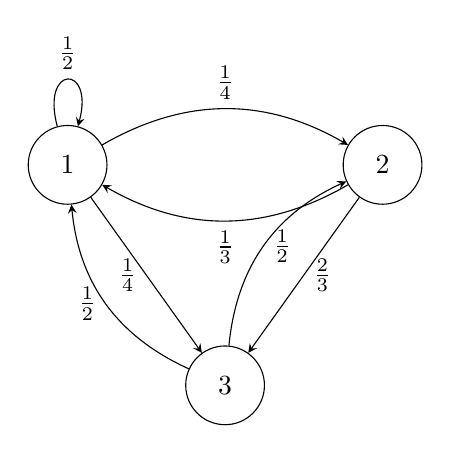
\begin{tikzpicture}[>=stealth, node distance=3cm]
    \node[circle,draw,minimum size=1cm] (1) at (0,0) {1};
    \node[circle,draw,minimum size=1cm] (2) at (4,0) {2};
    \node[circle,draw,minimum size=1cm] (3) at (2,-2.8) {3};

    \draw[->,loop above] (1) to node[above] {\(\frac12\)} (1);
    \draw[->,bend left] (1) to node[above] {\(\frac14\)} (2);
    \draw[->,bend left] (2) to node[below] {\(\frac13\)} (1);
    \draw[->] (1) to node[left] {\(\frac14\)} (3);
    \draw[->] (2) to node[right] {\(\frac23\)} (3);
    \draw[->,bend left] (3) to node[left] {\(\frac12\)} (1);
    \draw[->,bend left] (3) to node[right] {\(\frac12\)} (2);
\end{tikzpicture}
\end{center}

\subsection*{(b) Computing a Path Probability}

Suppose
\[
P(X_1=1)=P(X_1=2)=\frac14.
\]

Then
\[
P(X_1=3)=1-\frac14-\frac14=\frac12.
\]

Find
\[
P(X_1=3,X_2=2,X_3=1).
\]

Using the Markov property:
\[
P(X_1=3,X_2=2,X_3=1)
=
P(X_3=1\mid X_2=2)P(X_2=2\mid X_1=3)P(X_1=3).
\]

From the transition matrix:
\[
P(X_3=1\mid X_2=2)=p_{21}=\frac13,
\]
\[
P(X_2=2\mid X_1=3)=p_{32}=\frac12,
\]
and
\[
P(X_1=3)=\frac12.
\]

Therefore,
\[
P(X_1=3,X_2=2,X_3=1)
=
\frac13\cdot\frac12\cdot\frac12
=
\frac{1}{12}.
\]

\[
\boxed{P(X_1=3,X_2=2,X_3=1)=\frac{1}{12}.}
\]

\subsection*{(c) Irreducibility}

This chain is irreducible because every state can reach every other state.

For example:
\[
1\to 2,\quad 1\to 3,
\]
\[
2\to 1,\quad 2\to 3,
\]
\[
3\to 1,\quad 3\to 2.
\]

So all states communicate.

\[
\boxed{\text{The chain is irreducible.}}
\]

\subsection*{(d) Aperiodicity}

State 1 has a self-loop:
\[
p_{11}=\frac12>0.
\]

So state 1 can return to itself in one step.

In an irreducible chain, if one state is aperiodic, then all states are aperiodic.

\[
\boxed{\text{The chain is aperiodic.}}
\]

\subsection*{(e) Stationary Distribution}

Let
\[
\pi=(\pi_1,\pi_2,\pi_3).
\]

The stationary distribution satisfies
\[
\pi P=\pi,
\]
and
\[
\pi_1+\pi_2+\pi_3=1.
\]

Solving
\[
(\pi_1,\pi_2,\pi_3)
\begin{pmatrix}
\frac12 & \frac14 & \frac14\\
\frac13 & 0 & \frac23\\
\frac12 & \frac12 & 0
\end{pmatrix}
=
(\pi_1,\pi_2,\pi_3),
\]
gives
\[
\boxed{
\pi=
\left(\frac{12}{31},\frac{9}{31},\frac{10}{31}\right).
}
\]

\subsection*{(f) Is It a Limiting Distribution?}

The chain is:

\begin{itemize}
    \item irreducible,
    \item positive recurrent, because it is finite and irreducible,
    \item aperiodic.
\end{itemize}

Therefore it is ergodic, and the stationary distribution is also the limiting distribution.

So
\[
\boxed{
\lim_{n\to\infty}P^n
=
\begin{pmatrix}
\pi\\
\pi\\
\pi
\end{pmatrix}
}
\]
where
\[
\pi=
\left(\frac{12}{31},\frac{9}{31},\frac{10}{31}\right).
\]

\section{Three-State Chain With Equal Switching}

Consider a system with states
\[
0,1,2.
\]

Every hour, the system moves to a different state, chosen by a fair coin-like mechanism. From each state, it moves to one of the other two states with probability \(1/2\) each.

The transition matrix is
\[
P=
\begin{pmatrix}
0 & \frac12 & \frac12\\
\frac12 & 0 & \frac12\\
\frac12 & \frac12 & 0
\end{pmatrix}.
\]

\subsection*{Transition Diagram}

\begin{center}
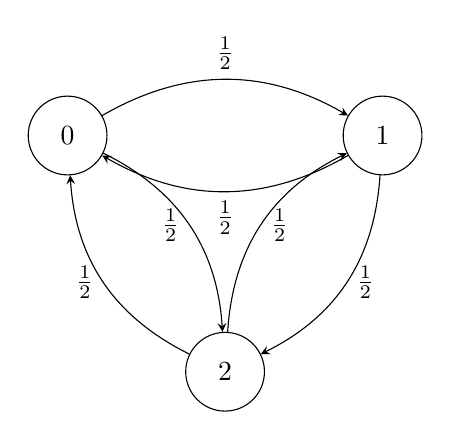
\begin{tikzpicture}[>=stealth, node distance=3cm]
    \node[circle,draw,minimum size=1cm] (0) at (0,0) {0};
    \node[circle,draw,minimum size=1cm] (1) at (4,0) {1};
    \node[circle,draw,minimum size=1cm] (2) at (2,-3) {2};

    \draw[->,bend left] (0) to node[above] {\(\frac12\)} (1);
    \draw[->,bend left] (1) to node[below] {\(\frac12\)} (0);
    \draw[->,bend left] (0) to node[left] {\(\frac12\)} (2);
    \draw[->,bend left] (2) to node[left] {\(\frac12\)} (0);
    \draw[->,bend left] (1) to node[right] {\(\frac12\)} (2);
    \draw[->,bend left] (2) to node[right] {\(\frac12\)} (1);
\end{tikzpicture}
\end{center}

\subsection*{Stationary Distribution}

Because the chain is symmetric, each state has the same long-run probability.

So
\[
\pi_0=\pi_1=\pi_2.
\]

Since probabilities add to 1:
\[
\pi_0+\pi_1+\pi_2=1.
\]

Thus,
\[
3\pi_0=1.
\]

Therefore,
\[
\pi_0=\pi_1=\pi_2=\frac13.
\]

So
\[
\boxed{
\pi=\left(\frac13,\frac13,\frac13\right).
}
\]

\subsection*{Aperiodicity}

There are no self-loops, so the chain cannot return in one step.

But state 0 can return to itself in 2 steps:
\[
0\to 1\to 0.
\]

It can also return in 3 steps:
\[
0\to 1\to 2\to 0.
\]

Since
\[
\gcd(2,3)=1,
\]
the period is 1.

Therefore, the chain is aperiodic.

The chain is finite, irreducible, and aperiodic, so it has a limiting distribution equal to the stationary distribution.

\section{Queuing Systems}

A queueing system studies waiting lines.

Examples:
\begin{itemize}
    \item customers waiting at a bank,
    \item patients waiting at a hospital,
    \item calls waiting in a call center,
    \item jobs waiting to be processed by a machine.
\end{itemize}

Queueing is not mainly an optimization process. It is mainly used to measure and understand efficiency, especially waiting time and service capacity.

\section{Elements of a Queue}

\[
\begin{array}{|c|p{10cm}|}
\hline
\textbf{Element} & \textbf{Meaning}\\
\hline
\text{Customer} & The person, item, call, or job arriving for service.\\
\hline
\text{Server} & The person or machine giving service. There may be one server or many servers.\\
\hline
\text{Interarrival time} & Time between two successive arrivals.\\
\hline
\text{Service time} & Time taken by the server to serve one customer.\\
\hline
\end{array}
\]

\section{Queue Size, Queue Discipline, and Customer Behaviour}

\[
\begin{array}{|c|p{10cm}|}
\hline
\textbf{Term} & \textbf{Meaning}\\
\hline
\text{Queue size} & Maximum number of customers that the queue can hold. It may be finite or infinite.\\
\hline
\text{Queue discipline} & The rule used to select the next customer for service.\\
\hline
\text{Source} & The population from which customers come. It may be finite or infinite.\\
\hline
\end{array}
\]

Common queue disciplines:

\[
\begin{array}{|c|p{10cm}|}
\hline
\textbf{Discipline} & \textbf{Meaning}\\
\hline
\text{FCFS/FIFO} & First come, first served. This is the most common.\\
\hline
\text{LCFS/LIFO} & Last come, first served.\\
\hline
\text{SIRO} & Service in random order.\\
\hline
\text{Priority} & Some customers are served before others based on priority.\\
\hline
\end{array}
\]

Customer behaviour in queues:

\[
\begin{array}{|c|p{10cm}|}
\hline
\textbf{Behaviour} & \textbf{Meaning}\\
\hline
\text{Jockeying} & Changing from one queue to another queue to reduce waiting time.\\
\hline
\text{Balking} & Not joining the queue because it looks too long.\\
\hline
\text{Reneging} & Joining the queue first, but leaving before service because the wait is too long.\\
\hline
\end{array}
\]

\section{Role of the Exponential Distribution in Queueing}

In many queueing models, arrivals are assumed to occur randomly. Therefore, the interarrival time is often modeled as exponential.

If
\[
T\sim \operatorname{Exponential}(\lambda),
\]
then
\[
f(t)=\lambda e^{-\lambda t},\qquad t>0.
\]

The expected interarrival time is
\[
E[T]=\frac{1}{\lambda}.
\]

The cumulative probability is
\[
P(T\leq A)=1-e^{-\lambda A}.
\]

The probability of no arrival during a period of length \(A\) is
\[
P(T>A)=e^{-\lambda A}.
\]

\section{Memoryless Property}

The exponential distribution has the memoryless property:

\[
P(T>T+s\mid T>s)=P(T>T).
\]

Using different letters to avoid confusion, write it as
\[
P(X>a+b\mid X>b)=P(X>a).
\]

This means:

\begin{center}
\textit{If you have already waited \(b\) units of time, the remaining waiting time behaves like a fresh new waiting time.}
\end{center}

\subsection*{Proof}

\[
P(X>a+b\mid X>b)
=
\frac{P(X>a+b,\;X>b)}{P(X>b)}.
\]

If \(X>a+b\), then automatically \(X>b\). So
\[
P(X>a+b,\;X>b)=P(X>a+b).
\]

Thus,
\[
P(X>a+b\mid X>b)
=
\frac{P(X>a+b)}{P(X>b)}.
\]

For an exponential random variable,
\[
P(X>x)=e^{-\lambda x}.
\]

Therefore,
\[
P(X>a+b\mid X>b)
=
\frac{e^{-\lambda(a+b)}}{e^{-\lambda b}}
=
e^{-\lambda a}.
\]

But
\[
P(X>a)=e^{-\lambda a}.
\]

Hence,
\[
\boxed{
P(X>a+b\mid X>b)=P(X>a).
}
\]

\section{Example: Machine Failure Claim}

A machine fails on average once every 5 hours. Then the failure rate is
\[
\lambda=\frac{1}{5}=0.2
\]
per hour.

The time to failure is
\[
T\sim \operatorname{Exponential}(0.2).
\]

Suppose an operator says the machine breaks down every night around 8:30 PM.

This claim is not supported by the exponential model because the exponential time to failure is random and memoryless.

For example, if the current time is 8:20 PM, then there are only 10 minutes until 8:30 PM.

Convert:
\[
10\text{ minutes}=\frac{10}{60}=\frac16\text{ hour}.
\]

The probability of failure by 8:30 PM is
\[
P\left(T\leq \frac16\right)
=
1-e^{-0.2(1/6)}.
\]

\[
=1-e^{-1/30}
\approx 0.0328.
\]

This is small, so the model does not support the claim that failure happens regularly at 8:30 PM.

\section{Pure Birth Model}

A pure birth model is a model where only arrivals occur.

There are no departures or deaths.

Let
\[
p_n(t)=P(\text{exactly }n\text{ arrivals occur during time }t).
\]

Then
\[
p_0(t)=P(\text{no arrivals during time }t).
\]

For a Poisson process with rate \(\lambda\),
\[
p_0(t)=e^{-\lambda t}.
\]

\subsection*{Small Interval Approximation}

For a very small interval \(h>0\):

\[
p_0(h)=e^{-\lambda h}.
\]

Using Taylor expansion,
\[
e^{-\lambda h}
=
1-\lambda h+\frac{(\lambda h)^2}{2!}-\cdots.
\]

For very small \(h\), terms involving \(h^2,h^3,\ldots\) are very small.

So
\[
p_0(h)\approx 1-\lambda h.
\]

Also,
\[
p_1(h)\approx \lambda h.
\]

The probability of two or more arrivals in a very small interval \(h\) is negligible.

\subsection*{Difference-Differential Equations}

For \(n>0\),
\[
p_n(t+h)\approx p_n(t)(1-\lambda h)+p_{n-1}(t)\lambda h.
\]

Interpretation:

\begin{itemize}
    \item First part: \(n\) arrivals happened by time \(t\), and no arrival occurs in the small interval \(h\).
    \item Second part: \(n-1\) arrivals happened by time \(t\), and one arrival occurs in the small interval \(h\).
\end{itemize}

For \(n=0\),
\[
p_0(t+h)\approx p_0(t)(1-\lambda h).
\]

Taking limits as \(h\to 0\), we get
\[
p_n'(t)=-\lambda p_n(t)+\lambda p_{n-1}(t),\qquad n>0,
\]
and
\[
p_0'(t)=-\lambda p_0(t).
\]

Solving these equations gives
\[
\boxed{
p_n(t)=e^{-\lambda t}\frac{(\lambda t)^n}{n!},\qquad n=0,1,2,\ldots
}
\]

This is the Poisson distribution with mean \(\lambda t\).

\section{Exponential Versus Poisson}

\[
\begin{array}{|c|c|c|}
\hline
 & \textbf{Exponential} & \textbf{Poisson}\\
\hline
\text{Random variable} & \text{Time between events} & \text{Number of events in time }t\\
\hline
\text{Range} & t\geq 0 & n=0,1,2,\ldots\\
\hline
\text{Main formula} & f(t)=\lambda e^{-\lambda t} & p_n(t)=e^{-\lambda t}\frac{(\lambda t)^n}{n!}\\
\hline
\text{Mean} & \frac{1}{\lambda} & \lambda t\\
\hline
\end{array}
\]

\section{Pure Death Model}

A pure death model is a model where only departures or deaths occur.

Suppose we start with \(N\) individuals.

Let
\[
p_n(t)=P(\text{there are }n\text{ individuals left at time }t).
\]

Deaths occur at rate \(\mu\).

The pure death model leads to a truncated Poisson distribution:

\[
\boxed{
p_n(t)=\frac{(\mu t)^{N-n}e^{-\mu t}}{(N-n)!},
\qquad n=1,2,\ldots,N.
}
\]

Here \(N-n\) is the number of deaths that have occurred by time \(t\).

The probability of reaching zero is
\[
\boxed{
p_0(t)=1-\sum_{n=1}^{N}p_n(t).
}
\]

This is called truncated because the population cannot go below zero.

\section{Birth and Death Models}

\[
\begin{array}{|c|c|}
\hline
\textbf{Model} & \textbf{Meaning}\\
\hline
\text{Pure birth model} & Only arrivals or births occur.\\
\hline
\text{Pure death model} & Only departures or deaths occur.\\
\hline
\text{Birth-death model} & Both arrivals and departures can occur.\\
\hline
\end{array}
\]

In queueing:

\begin{itemize}
    \item arrivals are like births,
    \item service completions are like deaths.
\end{itemize}

So queueing systems can often be modeled using birth-death processes.

\section{End-of-Lecture Essay Questions and Answers}

\subsection*{Question 1}

Explain how a Poisson process can be constructed using exponential interarrival times.

\textbf{Answer.}

Let \(T_1,T_2,\ldots\) be independent exponential random variables with rate \(\lambda\). These represent waiting times between consecutive events. Define
\[
S_n=T_1+\cdots+T_n.
\]
Then \(S_n\) is the time of the \(n\)th event. The counting process is
\[
N(t)=\max\{n:S_n\leq t\}.
\]
This counts how many events have occurred by time \(t\). This construction gives a Poisson process with rate \(\lambda\).

\subsection*{Question 2}

Explain why
\[
P(S_n>t)=P(N(t)<n).
\]

\textbf{Answer.}

\(S_n>t\) means the \(n\)th event has not occurred by time \(t\). Therefore, fewer than \(n\) events have occurred by time \(t\). That is exactly the event \(N(t)<n\). Hence,
\[
P(S_n>t)=P(N(t)<n).
\]
Since \(N(t)\sim\operatorname{Poisson}(\lambda t)\), this becomes
\[
P(S_n>t)=\sum_{j=0}^{n-1}e^{-\lambda t}\frac{(\lambda t)^j}{j!}.
\]

\subsection*{Question 3}

Cars arrive at rate 12 per hour. Each car stops with probability \(1/4\). You are third in line. Find the probability that you wait more than 1 hour.

\textbf{Answer.}

The useful car rate is
\[
\lambda=12\left(\frac14\right)=3
\]
per hour.

Since you are third in line, you need the third useful car. Your waiting time is \(S_3\).

We need
\[
P(S_3>1)=P(N(1)<3).
\]

Since
\[
N(1)\sim\operatorname{Poisson}(3),
\]
we get
\[
P(S_3>1)=P(N(1)=0)+P(N(1)=1)+P(N(1)=2).
\]

\[
=e^{-3}+3e^{-3}+\frac{3^2}{2!}e^{-3}.
\]

\[
=e^{-3}\left(1+3+\frac92\right).
\]

\[
\boxed{
P(S_3>1)=\frac{17}{2}e^{-3}.
}
\]

\subsection*{Question 4}

State and prove the memoryless property of the exponential distribution.

\textbf{Answer.}

If \(X\sim\operatorname{Exponential}(\lambda)\), then
\[
P(X>a+b\mid X>b)=P(X>a).
\]

Proof:
\[
P(X>a+b\mid X>b)
=
\frac{P(X>a+b,\;X>b)}{P(X>b)}.
\]
Since \(X>a+b\) implies \(X>b\),
\[
P(X>a+b,\;X>b)=P(X>a+b).
\]
Thus,
\[
P(X>a+b\mid X>b)
=
\frac{P(X>a+b)}{P(X>b)}.
\]
Using \(P(X>x)=e^{-\lambda x}\),
\[
\frac{P(X>a+b)}{P(X>b)}
=
\frac{e^{-\lambda(a+b)}}{e^{-\lambda b}}
=e^{-\lambda a}
=P(X>a).
\]
Therefore, the exponential distribution is memoryless.

\subsection*{Question 5}

Explain the difference between the exponential distribution and the Poisson distribution in the context of arrivals.

\textbf{Answer.}

The exponential distribution models waiting time. It answers questions such as: how long until the next customer arrives?

The Poisson distribution models counts. It answers questions such as: how many customers arrive in 1 hour?

If arrivals follow a Poisson process with rate \(\lambda\), then the time between arrivals is exponential with mean \(1/\lambda\), while the number of arrivals in time \(t\) is Poisson with mean \(\lambda t\).

\subsection*{Question 6}

Derive the pure birth probability
\[
p_n(t)=e^{-\lambda t}\frac{(\lambda t)^n}{n!}.
\]

\textbf{Answer.}

For a very small interval \(h\), the probability of no arrival is approximately
\[
1-\lambda h,
\]
and the probability of one arrival is approximately
\[
\lambda h.
\]
For \(n>0\),
\[
p_n(t+h)\approx p_n(t)(1-\lambda h)+p_{n-1}(t)\lambda h.
\]
Rearranging and taking \(h\to0\),
\[
p_n'(t)=-\lambda p_n(t)+\lambda p_{n-1}(t).
\]
For \(n=0\),
\[
p_0'(t)=-\lambda p_0(t).
\]
Solving this system gives
\[
p_n(t)=e^{-\lambda t}\frac{(\lambda t)^n}{n!}.
\]
Thus the pure birth model produces the Poisson distribution.

\subsection*{Question 7}

Explain the idea of a pure death model and why it gives a truncated Poisson distribution.

\textbf{Answer.}

In a pure death model, we start with a fixed number \(N\) of individuals and only deaths occur. No new individuals enter the system. If \(p_n(t)\) is the probability that \(n\) individuals remain at time \(t\), then \(N-n\) deaths have occurred by time \(t\). The probability has the form
\[
p_n(t)=\frac{(\mu t)^{N-n}e^{-\mu t}}{(N-n)!},
\qquad n=1,\ldots,N.
\]
It is called truncated because the number of deaths cannot exceed \(N\), and the population cannot go below zero.

\end{document}
